\documentclass[a4paper,11pt,danish]{article}

\usepackage[latin1]{inputenc}
\usepackage[T1]{fontenc}
\usepackage[danish]{babel}
\usepackage{url}
\usepackage{lastpage}
\usepackage{bookmark}
\usepackage{fancyhdr}
\usepackage{charter}
\usepackage{rotating}
\usepackage{pdflscape}
\usepackage{appendix}
\pagestyle{fancy}


\date{27. marts 2009}

\newcommand{\mytitle}{Eksamensopgave}
\newcommand{\mysubject}{Menneske-datamaskine interaktion (HCI)}

\newcommand{\HCI}{menneske-datamaskine interaktion}

\newcommand{\mycpr}{180387-1619}

\newcommand{\email}[1]{\href{mailto:#1}{\texttt{#1}}}

\renewcommand{\sectionmark}[1]{\markright{\thesection.\ #1}}

\renewcommand{\appendixtocname}{Bilag}
\renewcommand{\appendixpagename}{Bilag}
\renewcommand{\appendixname}{Bilag}


\title{\huge \mysubject \\ \normalsize \mytitle}

\author{
\begin{tabular}{lr}
  Navn & Julian M�ller \\
  CPR-nummer & 180387-1619 \\
  di-nummer & di080047 \\
  E-mail & \email{di080047@diku.dk} \\
\end{tabular}
}

\fancyhead{}

 	\lhead{}
 	\chead{}
 	\rhead{}
 	\lfoot{}
 	\cfoot{}
 	\rfoot{}

\fancyhead[L]{HCI: \mytitle}
\fancyhead[C]{Julian M�ller}
\fancyhead[R]{\mycpr}
\fancyfoot[L]{\rightmark}
\fancyfoot[R]{Side \thepage \ af \pageref{LastPage}}

\begin{document}

\maketitle
\tableofcontents

\pagebreak

%%% Local Variables: 
%%% mode: latex
%%% TeX-master: "julian_moeller_eksamen"
%%% End: 

\section{Kursusaktivitet dokumenteret ved syv ugeopgaver}
\label{sec:kurs-dokum-ved}

De syv ugeopgaver kan findes i de vedlagte bilag (s. \pageref{sec:ugeopgaver}).

Overordnet set er jeg ret tilfreds med mine ugeopgaver. Jeg synes jeg
er kommet godt rundt omkring de stillede krav i alle opgaverne, og har
f�et udf�rt nogle gode analyser og forbedringsforslag.

Aspekterne, jeg generelt ikke har v�ret helt tilfreds med i mine
opgaver har v�ret de forskellige brugerunders�gelser. Jeg synes det
var sv�rt at retf�rddigg�re s� ``store'' unders�gelser for s� sm�
opgaver. Jeg synes ikke at den store m�ngde tid det ville tage fx at
lave en komplet kontekstuel unders�gelse var retf�rdiggjort - hverken
for mig selv eller for testpersonerne. Fra et teoretisk synsspunkt
kunne jeg godt have brugt mere tid p� unders�gelserne, for at f� et
mere repr�sentativt resultat.

Den unders�gelse jeg var mest tilfreds med, er at finde i min
ugeopgave 4, som ogs� er den opgave jeg er mest tilfreds med. Opgaven
var sp�ndende og ved hj�lp af unders�gelsen og de to stillede konkrete
scenarier fandt jeg nogle gode krav til det �nskede rejsesystem inden
for \emph{PACT}. Den kontekstuelle unders�gelse lagde ogs� et godt
grundlag for det konkrete scenarie der skulle skrives. Endvidere blev
mit endelige redesigforslag vellykket og passede godt til den stillede
opgave samt de forskellige brugsscenarier der var.

Det svageste punkt ved min opgave var den gennemg�ende mangel p�
referencer jeg har f�et lavet i mine ugeopgaver. I retrospekt ville
flere referencer til l�reb�ger, artikler eller lignende have gavnet opgaven,
da det dermed ville have v�ret tydeligere at mine id�er ikke blot var
grebet ud af den bl� luft, men byggede p� videnskabelig forskning
inden for \HCI.


\section{Analyse og redesign af webside}
\label{sec:analyse-og-redesign}

Da jeg i min ugeopgave 6 besk�ftigede mig med AVIS biludlejnings
webside, er det ogs� den, jeg vil besk�ftige mig med her. Websiden er
at finde p� \url{http://www.avis.dk}.


\subsection{PACT-analyse af \texttt{ww.avis.dk}}
\label{sec:pact-analyse-af-avisdk}

\subsubsection{People}
\label{sec:people}

Brugerne af AVIS' webside vil prim�rt v�re personer, der skal v�re
chauff�rer i de lejede biler. Da billejere skal v�re over 21 �r
\cite{web-lejebetingelser}, m� det antages at der formentlig ikke
mange b�rn eller unge der vil benytte AVIS' webside. Derudover
forestiller jeg mig at st�rstedelen af billejere er under
pensionsalderen.

Der kan sagtens forekomme farveblinde brugere, men st�rkt syns- eller
fysisk handicappede forekommer formentlig ikke. De fysisk
handicappede, der har k�rekort har oftest brug for speciallavede
biler, der fx udelukkende kan styres med h�nderne. Da markedet for
specielle handicapbiler s� lille og priserne dermed antageligt meget
h�je, er sv�rt fysisk handicappede ikke en m�lgruppe for AVIS
biludlejning.

Da biludlejning kan forekomme ofte under ferier, vil der v�re en r�kke
brugere, der er turister og dermed sandsynligvis ikke forst�r dansk.

\subsubsection{Activities}
\label{sec:activities}

Det overordnede form�l med AVIS' webside er at leje en bil. Processen
foreg�r over en r�kke trin, hvori der skal v�lges udlejningsdatoer,
afhentnings- og afleveringssted, biltype o.l. Processen kr�ver ikke
samarbejde med andre, men kan naturligvis forekomme i selskab med
andre personer. Der er ingen sikkerhedsm�ssige aspekter i forbindelse
med selve udlejningsprocessen. Sikkerhed er dog stadig et aspekt, da
websiden vil bede om personf�lsom data.

Udlejningsprocessen vil oftest foreg� over en enkelt session, og
formentlig forekomme sj�ldent. Derfor skal det v�re let at finde al
den n�dvendige information omkring biludlejning (fx minimumalder, krav
til k�rekort, forsikring, ekstraudstyr).

Da udlejningen foreg�r via en webside er det vigtigt, at responstiden
er lav, s� brugerne ikke bliver forvirrede og/eller irriterede.

Der kan sagtens forekomme fejl under udlejningsprocessen (fx en bil
der �nskes afhentet p� et tidspunkt hvor udlejningskontoret er
lukket).

\subsubsection{Contexts}
\label{sec:contexts}

Udlejningsprocessen vil formentlig foreg� hjemmefra eller fra et
kontor og lyd og andre forstyrrende elementer er derfor ikke
med garanti socialt acceptable eller teknisk mulige.

Brugen af websiden kan forekomme p� alle tider af d�gnet.

Udlejningen kan eventuelt foreg� over en ret langsom
internetforbindelse.

Da udlejningen ikke finder sted p� et AVIS-kontor eller lignende, er
der ikke n�dvendigvis hj�lp at hente fra personer.


\subsubsection{Technologies}
\label{sec:technologies}

Der er tale om en webside, hvor der ikke skal tastes massive m�ngder
information ind. Derfor b�r st�rstedelen af navigationen i
udlejningsprocessen kunne klares vha. fx en mus.

Websidens servere skal have en h�j garanteret oppetid, da brug kan
forekomme p� alle tider af d�gnet.

Det er vigtigt at websidens indhold er opdateret, s� det er muligt at
se, hvilke biler der fx er til r�dighed ved et givent
udlejningskontor.

Da websiden skal tage imod personf�lsom data, er der behov for
kryptering af den data, der udveksles under \emph{browsing} af
websiden, men s� sandelig ogs� kryptering af de data der lagres i
AVIS' database til slut.
%%% Local Variables: 
%%% mode: latex
%%% TeX-master: "julian_moeller_eksamen"
%%% End: 

\subsection{Analyse af problemer ved AVIS' webside}
\label{sec:analyse-af-problemer}

\subsubsection{Affinitetsdiagram}
\label{sec:affinitetsdiagram}

I det til opgaveformuleringen vedlagte bilag D har jeg lokaliseret
gennemg�ende temaer i problempunkterne ved at anvende algoritmen p�
\cite[s. 483]{benyon}. Hermed fik jeg dannet et affinitetsdiagram, som
lettere gav et overbliv over kerneproblemerne p� AVIS' webside.

Diagrammet endte med at best� af to overpunkter: ``uoverskuelighed''
samt ``manglende information''. Problemerne i affinitetsdiagrammet er
ikke listet i prioriteret r�kkef�lge.

\begin{center}
  \begin{tabular}{ | c | p{5cm} | p{6cm} |}
    \multicolumn{3}{c}{\textbf{Uoverskuelighed}} \\

    \hline
    Nr. & Titel & Beskrivelse \\ \hline

    U1
    & Hj�lpelinks sv�re at finde 
    & AVIS' webside har en r�kke hj�lpelinks, men de er sv�re at finde,
      da de er placeret nederst p� siden
    \\ \hline

    U2
    & Uklar opdeling af information
    & Navigationslinksne i topmenuen har misvisende titler ift. de linkede
      siders indhold.
    \\ \hline

    U3
    & Hj�lpetekst til formularer misvisende
    & Fx st�r der, at der skal v�lges postnummer, hvilket blot resulterer i
      endnu et formularfelt, hvori land skal indtastes. Endvidere st�r det ikke
      angivet, at datofelterne p� s�geformularen netop er datofelter.
    \\ \hline

    U4
    & Navigation inkonsistent
    & Navigation via billeder resulterer i en side, der repr�senterer indholdet
      af billedet. Dette er dog ikke tilf�ldet p� biloversigten, hvor der linkes
      til forsiden.
    \\ \hline

    U5
    & S�gning efter udlejningskontorer forvirrende
    & Medmindre man er meget stedkendt, er der ikke nogen mulighed for at finde
      ud af hvor et udlejningskontor ligger, medmindre det lokaliseres andetsteds.
      Endvidere er der problemer, hvis man vil bestille en bil fra et center uden
      for �bningstid, da der ikke henvises til n�rmeste andet biludlejningskontor.
    \\ \hline

    U6
    & Tvivl om brug af knapper ved s�gning
    & Der er to knapper p� s�geformularen p� forsiden: ``Forts�t'' og ``F� et
      tilbud''. Der er tvivl hos brugerne om knappernes brug.
    \\ \hline
  \end{tabular}
\end{center}

\begin{center}
  \begin{tabular}{ | c | p{5cm} | p{6cm} |}
    \multicolumn{3}{c}{\textbf{Manglende information}} \\

    \hline
    Nr. & Titel & Beskrivelse \\ \hline

    M1
    & �bnings-, afleverings- og afhentningstider er ikke tydelige
    & Hvis man har fors�gt at leje en bil uden for et centers �bnignstid,
      f�r man blot at vide med en meget lys gr� skrift, at bilen kan afhentes
      p� et andet, givent tidspunkt. Informationen overses alts� let.
    \\ \hline

    M2
    & Alternative muligheder mangler
    & Hvis man har valgt et udlejningssted og/eller en bil, der ikke kan lade
      sig g�re, mangler der en automatisk visning af tilg�ngelige alternativer.
    \\ \hline

    M3
    & Regler o.l. er sv�re at finde
    & Dels er regler om fx minimumsalder sv�re at finde, da de gemmer sig p� en
      underside til et af linksne i bunden af websiden. Desuden bliver der ikke
      gjort opm�rksom p� eventuelt g�ldende regler undervejs i bestillingen af 
      en lejebil.
    \\ \hline

    M4
    & Fejlbeskeder mangler og/eller er misvisende
    & Mange af fejlbeskederne g�r ikke opm�rksom p� deres grund til at blive vist,
      s� brugeren har kun lille mulighed for at rette eventuelle fejl.
    \\ \hline

    M5
    & Bilbeskrivelser sv�re at differentiere
    & Oversigten over tilg�ngelige biltyper g�r det ikke let at differentiere
      mellem forskellige biltyper. Fx er der ikke nogen enkel m�de at finde de biler,
      der har 6 s�der, bortset fra manual gennems�gning af alle biltyper.
    \\ \hline

  \end{tabular}
\end{center}

Som det kan ses af de to ovenst�ende tabeller, er de prim�re problemer
p� AVIS' webside af kommunikationskarakter. Dvs., at de repr�senterer
fejl og mangler, som brugeren har behov for at se, for at kunne
foretage en tryg og velovervejet bestilling.

\subsubsection{Korrelation mellem analyse/teori og diagram}
\label{sec:korr-mell-analys}

I PACT-analysen blev der lagt op til at leje af bil via websiden
prim�rt ville foreg� alene, dvs. uden hj�lpeansatte til r�dighed o.l
(afsnit \ref{sec:contexts}). Derfor er det meget vigtigt, at AVIS'
webside g�r alt hvad den kan for at g�re det let for brugerne selv at
finde den information de s�ger efter. Dette muligg�r AVIS' webside dog
ikke ordentligt.

Dermed lever AVIS' webside heller ikke op til f�lgende af Nielsens
krav \cite[s. 26]{nielsen}:

\begin{itemize}
\item \emph{Learnability} \\
  Systemet er forvirrende og mangler
  information, s� nye brugere har sv�rt ved at komme i gang
\item \emph{Errors} \\
  Der kan nemt forekomme fejl under brugen, og hj�lpen til at
  overkomme disse fejl er utilstr�kkelig
\item \emph{Satisfaction} \\
  Overordnet set er der en del, der direkte udtrykker irritation ved
  brug af AVIS' webside. Kombineres dette med de mange fejl omkring
  kommunikation og information er resultatet ikke flatterende.
\end{itemize}
\subsection{Making use of business goals in usability evaluation}
\label{sec:making-use-business}

Artiklen af Hornb�k og Fr�kj�r \cite{makeuseofbus} viser, at et �get
fokus p� forretningsm�l fra unders�geren giver et st�rre fokus p�
relevante problemer. Problemerne omhandler mere specifikt de
kerneomr�der virksomheden har med den unders�gte service og er dermed
bedre som fokuspunkter til at udbedre eventuelle
brugsproblemer. Evalueringer, der indeholdt f�rre problempunkter,
inkluderede oftere relevante problemer end de evalueringer, der havde
mange problempunkter.


\begin{quote}
  Another explanation might be that business goals help focus the
  evaluation. Problems reported in the BG-TA condition are generally
  longer than in the TA condition.\\
  \ldots \\
  Thus, being prompted to
  consider business goals from the onset of an evaluation may have the
  psychological effect of tuning evaluators' work toward these goals
  and helping them understand which feedback the Company would
  appreciate.
\end{quote}

Det konkluderes endvidere, at en fornyelse af en velkendt
evalueringsteknik alts� har vist sig at v�re mere effektiv end den
g�ngse fremgangsm�de med at udvikle helt nye evalueringsmetoder for at
fremme brugbarheden af evalueringerne.

\begin{quote}
  It is noteworthy that the effect of making use of business goals in
  terms of downstream utility is strong (30--42\%), more so than the
  effects typically obtained by new or improved evaluation techniques.
\end{quote}

Teknikken brugt i \cite{makeuseofbus} adskiller sig fra metoderne i
\cite[kapitel 12]{benyon} ved ikke direkte at omhandle de g�ngse m�l
for brugsvenlighed: overordnet brugsvenlighed, krav for
�vede brugere, krav for enkeltgangsbrugere, krav for sporadisk brug
samt till�ringsevne (eng: \emph{learnability}). I stedet fokuseres
unders�gelsen direkte p� virksomhedens m�l med servicen, og dermed kun
indirekte p� de klassiske brugsvenlighedskriterier.

Dette giver unders�geren et fokusomr�de, s� de fundne problemer er
specificeret omkring et brugbart m�l. I \cite{benyon} l�gges der
umiddelbart op til, at en unders�gelses vellykkethed afg�res af
antallet af funde problemer, hvadenten disse problemer er store eller
sm�, relevante eller ligegyldige. Dermed �ges virksomhedens resultat
fra unders�gelsen gevaldigt, da de vil opn� flere brugbare
problemerpunkter, som, hvis de bliver rettet op p�, vil vises direkte
ved opfyldelse af forretningsm�lene. Fokusomr�det vil ogs� g�re
unders�gerne bedre i stand til at vurdere hvor kritisk et problem er
ud fra virksomhedens synspunkt, i stedet for ud fra synspunkterne
givet i teorierne for \HCI.

Metoden i \cite{makeuseofbus} kan dog ogs� blot ses som en instans af
\emph{IMPACT}-modellen, hvor \emph{Metric}-delen er relevans i forhold
til virksomhedens forretningsm�l.

Fordelen ved at bruge en metode som \cite{makeuseofbus} er, at
unders�geren ikke beh�ver s�tte sig ind i en ny evalueringsmetode, men
blot kan g�re brug af en, vedkommende i forvejen er fortrolig
med. Dermed kan unders�gerens fortrolighed, og dermed sandsynligvis
ogs� problempunkternes brugbarhed, �ges. Det skyldes at de ikke
beh�ver v�re erfarne i fx alle de metoder, der er n�vnt i \cite[12.2,
12.3, 12.4, 12.5]{benyon}, men m�ske kan n�jes med en enkelt metode.

Selvom resultatet i sidste ende m�ske ville v�re det samme, er det
langt hurtigere og mere effektivt at specificere m�lene i en metode, i
stedet for at unders�geren skal till�re sig en ny teknik.


%%% Local Variables: 
%%% mode: latex
%%% TeX-master: "julian_moeller_eksamen"
%%% End: 

\appendix
\appendixpage
\addappheadtotoc

\label{appendix}

\section{Figurer}
\label{sec:figurer}

\begin{figure}[h]
  \centering
  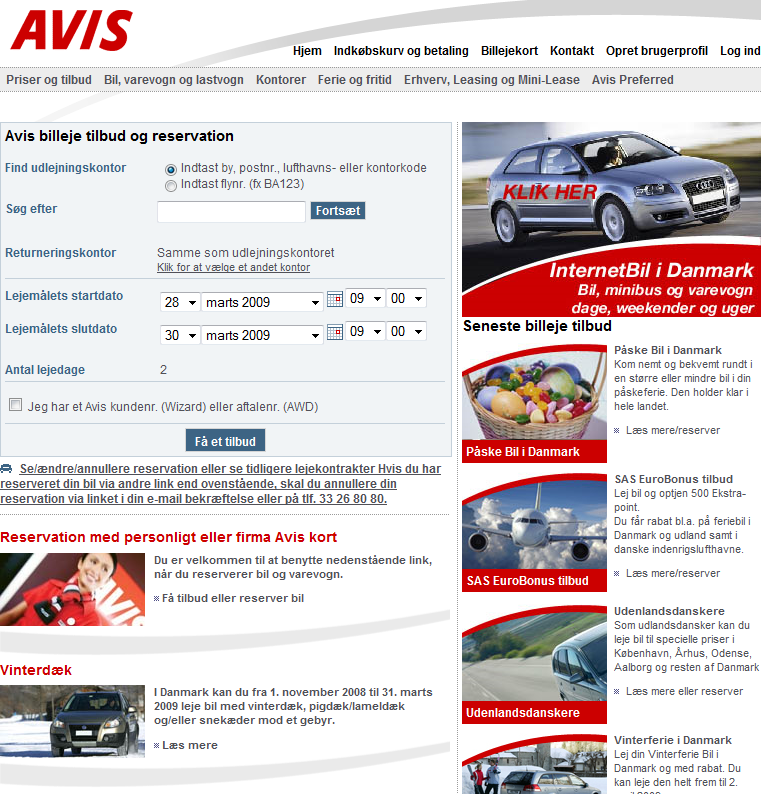
\includegraphics[width=13cm]{figures/avis_dk.png}
  \caption{AVIS' nuv�rende webside (marts 2009)}
  \label{fig:avisbilovs}
\end{figure}

\begin{figure}[h]
  \centering
  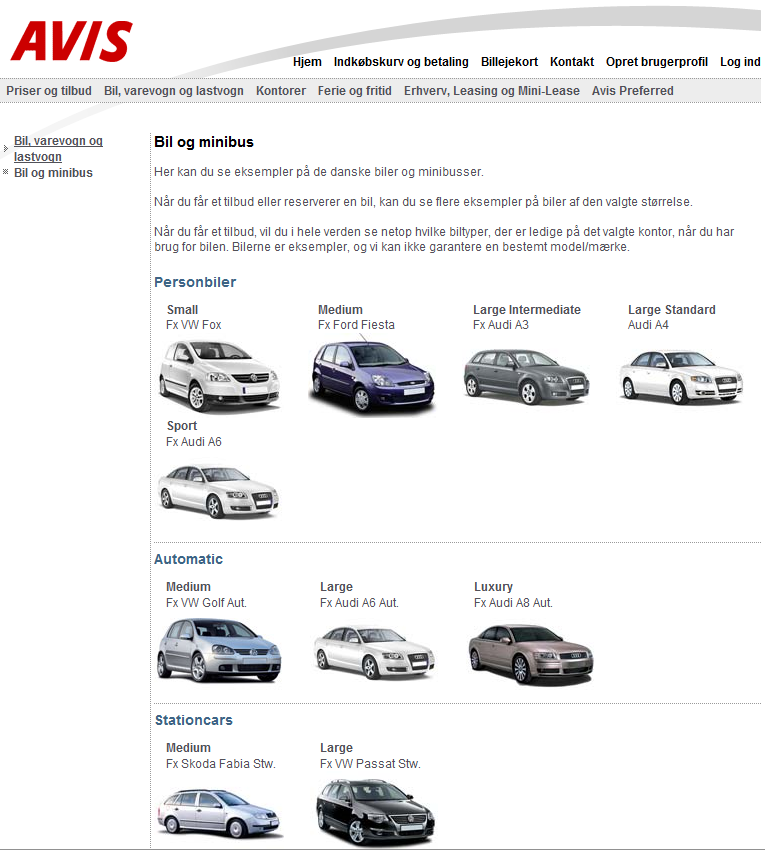
\includegraphics[width=13cm]{figures/avis_biloversigt.png}
  \caption{Biloversigten p� AVIS' nuv�rende webside (marts 2009)}
  \label{fig:avisdk}
\end{figure}

\begin{figure}[h]
  \centering
  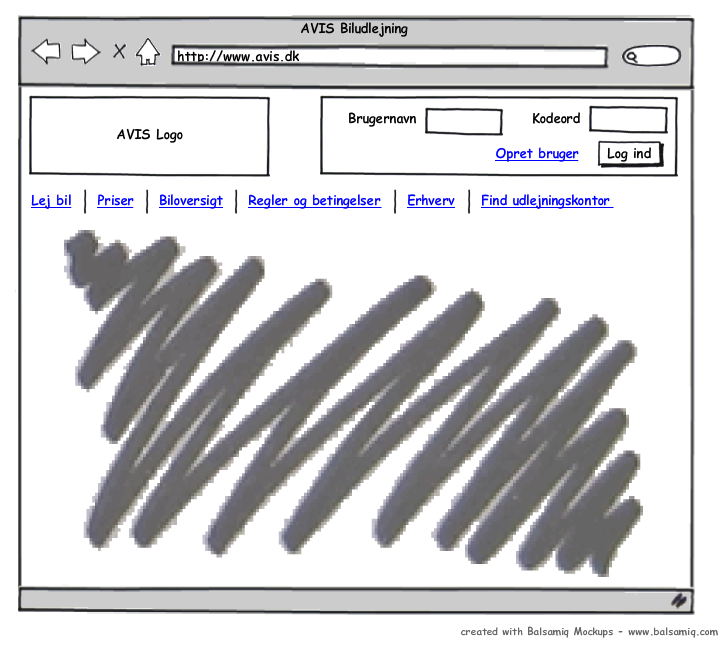
\includegraphics[width=13cm]{figures/menubar_mockup.png}
  \caption{Forslag til �ndring af menulinjen p� AVIS' webside}
  \label{fig:menubar}
\end{figure}

\begin{figure}[h]
  \centering
  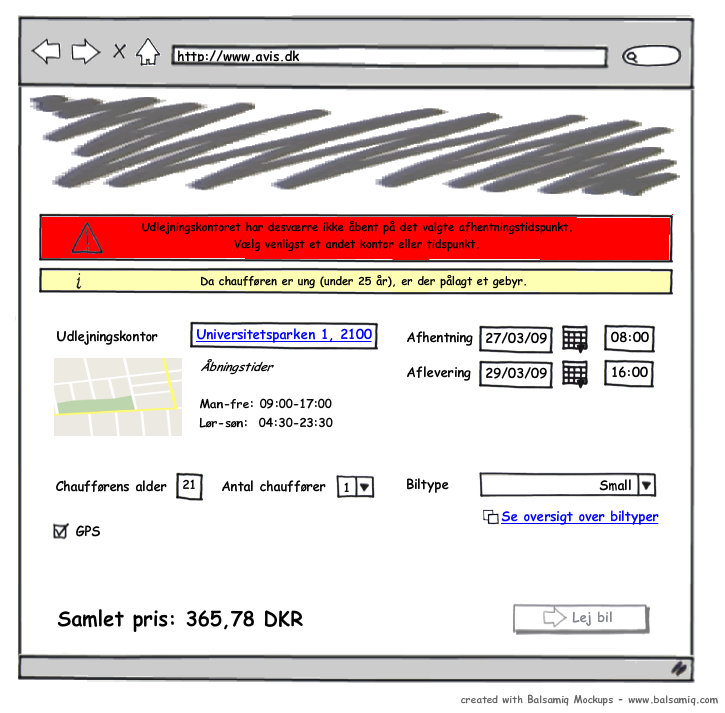
\includegraphics[width=13cm]{figures/search_mockup.png}
  \caption{Forslag til �ndring af s�geinterfacet p� AVIS' webside}
  \label{fig:search}
\end{figure}

\begin{figure}[h]
  \centering
  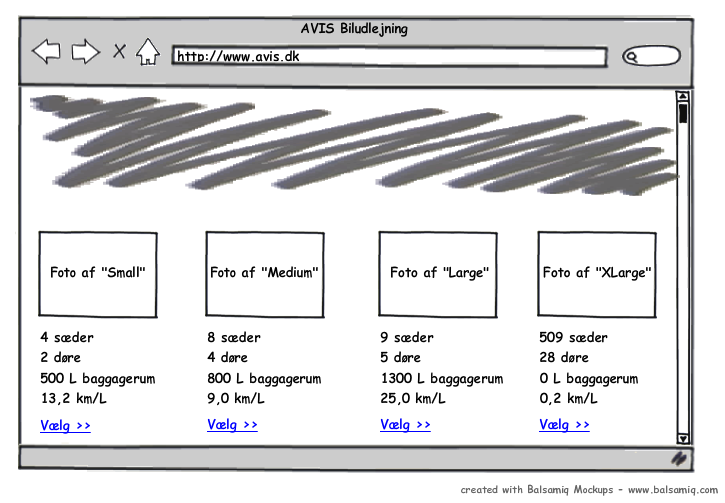
\includegraphics[width=13cm]{figures/choosecar_mockup.png}
  \caption{Forslag til �ndring af biloversigten p� AVIS' webside}
  \label{fig:choosecar}
\end{figure}

\clearpage


\section{Ugeopgaver}
\label{sec:ugeopgaver}


\end{document}